\documentclass[11pt]{article}
\usepackage[margin=1in,top=.91in,bottom=.92in,headheight=14pt]{geometry}
\usepackage[T1]{fontenc}\usepackage{lmodern}
\usepackage{graphicx,amsmath,amssymb,amsthm,booktabs,array,xcolor,hyperref,fancyhdr,microtype}
\definecolor{ink}{HTML}{18324A}\definecolor{accent}{HTML}{145D66}
\hypersetup{colorlinks=true,linkcolor=accent,urlcolor=accent,pdftitle={Three Riemann hypotheses in intuitionistic primitive recursive arithmetic}}
\pagestyle{fancy}\fancyhf{}\lhead{\small\textcolor{ink}{Riemann hypotheses in iPRA}}\rhead{\small\textcolor{ink}{Arithmetic and formalization}}\cfoot{\small\thepage}
\setlength{\parindent}{1.15em}\setlength{\parskip}{2pt}\renewcommand{\headrulewidth}{.3pt}
\newcommand{\N}{\mathbb N}\newcommand{\Z}{\mathbb Z}\newcommand{\Q}{\mathbb Q}\newcommand{\F}{\mathbb F}
\newcommand{\disc}{\operatorname{disc}}\newcommand{\RH}{\mathsf{RH}}\newcommand{\GRH}{\mathsf{GRH}}\newcommand{\ERH}{\mathsf{ERH}}
\newcommand{\ip}{\mathrm{iPRA}}\newcommand{\code}[1]{\texttt{\detokenize{#1}}}
\newtheorem{theorem}{Theorem}\newtheorem{lemma}[theorem]{Lemma}\newtheorem{proposition}[theorem]{Proposition}
\urlstyle{same}\raggedbottom
\begin{document}
\thispagestyle{plain}
\noindent{\sffamily\small\textcolor{accent}{MATHEMATICAL LOGIC \quad / \quad ANALYTIC NUMBER THEORY}}\par
\vspace{9pt}
\noindent{\LARGE\bfseries\color{ink} Three Riemann hypotheses in intuitionistic primitive recursive arithmetic\par}
\vspace{7pt}
\noindent{\large Complete splitting, Taylor coefficients and finite witnesses}\par
\vspace{5pt}\noindent{\small November 20, 2026}\par
\bigskip
A prime congruence test can express Dirichlet GRH with just one unbounded variable. For integers $m\ge2$, let $B_m(y)$ be the highest set-bit index of the product of all primes $p\le y$ congruent to $1$ modulo $m$, taking $B_m(y)=0$ for an empty product. Put $l=1+\lfloor\log_2(2n)\rfloor$. Then Dirichlet GRH is equivalent in the classical standard model to
\[
 \boxed{\quad \forall n\ge100\quad
   \max_{2\le m\le2n}|B_m(2n)-2B_m(n)|^2\le n(64l^2)^2.\quad}
\]
The formula quantifies over natural numbers, and its matrix is primitive recursive. For ordinary RH it suffices to use $m=2$, which selects the odd primes. For Dedekind ERH, select primes at which an input polynomial splits completely, and let the binary length $l$ control which polynomials enter the finite maximum. The same right side works in all three cases (Theorem~\ref{thm:split}).
\begin{center}\small
\begin{tabular}{@{}ll@{}}\toprule
Name in this report & Zeros in the open strip $0<\Re s<1$ lie on $\Re s=1/2$ for\\\midrule
RH & the Riemann zeta function $\zeta(s)$\\
Dirichlet GRH & every primitive Dirichlet $L(s,\chi)$, including complex characters\\
Dedekind ERH & $\zeta_K(s)$ for every number field $K$, including non-Galois fields\\\bottomrule
\end{tabular}
\end{center}
A second characterization reconstructs Taylor coefficients of a Dirichlet series from finite integer sums. Disks centered at $4+2^i$ already detect every possible off-line zero. A third replaces Mertens sums with Liouville sums or, more generally, sums along perfect powers, with an explicit conversion of the required growth constants. The object-theoretic proofs also convert a failing five-parameter Dedekind test into the least failing search radius and recover a failed tuple from that radius.
\paragraph{Proof strength.}
A closed term of type \code{Fm PTm 0} specifies an arithmetic conjecture. A Lean term of type \code{Prf PRAAx [] (Fm.iff A B)} proves a biconditional \emph{in} iPRA. A theorem about \code{naturalTerms.Holds} verifies an interpretation in the ordinary natural numbers. The identification of these arithmetic statements with complex zero statements uses the analytic theorems and proofs given in the text. The construction proves equivalences and supplies conditional algorithms; the three zero hypotheses remain open.
\newpage

\section*{Reading guide}\pdfbookmark[1]{Reading guide}{guide}
The first two input archives share the same polynomial prime-power test. The second also contains witness, determinant, energy, Farey and divisor-sum formulations. The present development retains those results and adds the following five groups. Section~\ref{sec:sentence} first fixes the common arithmetic notation.
\begin{center}\small
\begin{tabular}{@{}>{\raggedright\arraybackslash}p{.25\linewidth}>{\raggedright\arraybackslash}p{.32\linewidth}>{\raggedright\arraybackslash}p{.35\linewidth}@{}}\toprule
New material & Change in the mathematical data & Proof supplied\\\midrule
Complete splitting, \S\ref{sec:split} & One residue class, or just the primes at which all roots are rational modulo $p$. & Literal formulas and Lean readings. Prime-ideal comparison and passage to arbitrary subfields on paper.\\[4pt]
Taylor disks, \S\ref{sec:taylor} & Signed integer approximants at real centers, with a prescribed error for every coefficient. & Lean readings for all nine formulas. Analytic characterization, overlap identity and evaluation modulus on paper.\\[4pt]
Perfect powers, \S\ref{sec:powerdivisor} & Changes the sequence being summed, including $\mu$ to $\lambda$ and all orders $h\ge2$ at once. & Lean proofs of inversion, witness bounds and the ordinary Liouville equivalence. Residue transport on paper.\\[4pt]
A single search radius, \S\ref{sec:unary-cube} & One radius tests all inputs jointly. A bad radius produces an explicit field code and cutoff. & Empty-context object iPRA derivations in both directions, including the first dirty radius.\\[4pt]
Symmetric prefix tests, \S\ref{sec:symmetric-prefixes} & High powers, exponential sums, signs of polynomial coefficients, and a multiplicative certificate. & Lean finite equivalences and standard readings. The multiplicative certificate has an internal iPRA biconditional.\\\bottomrule
\end{tabular}
\end{center}
\paragraph{Earlier criteria retained.}
Sections~\ref{sec:kernel}--\ref{sec:verified} develop the prime-power test, its correspondence to the complex zero sets and its internal hierarchy. Sections~\ref{sec:audits}--\ref{sec:lagarias} treat prefix counts, arithmetic slack, integer probes, sparse cutoffs, smoothing, determinants, gcd energy, Farey discrepancies, dyadic series and the Lagarias divisor-sum criterion. The appendices give the Mertens bridges for the three families.
\paragraph{Which constructive reading to choose.}
A universal prime test specifies its full error allowance and admits a finite failure certificate. The Mertens versions ask for a bound for every prescribed exponent, and their explicit witness conversions matter in iPRA. The Taylor versions provide local rational evaluations at any requested precision from the prescribed coefficient bounds. These descriptions support different uses of the conjectures. Their standard classical equivalence alone does not produce an internal transformation between every pair of witnesses.

\paragraph{Application to the new number-theoretic tests.}
The module \code{UniversalCriteria.lean} also applies the finite-cube construction of Section~\ref{sec:unary-cube} directly to the Taylor, splitting and symmetric-prefix syntax. For example, for each of the nine Taylor sentences iPRA proves equivalence to every scheduled finite-cube test of that section. From an explicitly failed Taylor tuple it derives the least dirty radius, and from that radius it recovers a failed tuple. These derivations inspect just the syntax of the arithmetic matrix; their interpretation as detecting poles uses Theorem~\ref{thm:taylor}.

\newpage
\section{The arithmetic sentence}\label{sec:sentence}
The numerical sort is \(\N=\{0,1,\ldots\}\). Set \(d=d_0+1\), \(b=H+2\), and \(n=t+100\). For \(w\in\N\), put \([w]_{b,i}=\lfloor w/b^i\rfloor\bmod b\). The four polynomial parameters name
\[
 F=X^d+\sum_{i=0}^{d-1}([u]_{b,i}-[v]_{b,i})X^i .
\]
Ordinary signed subtraction in this display describes a pair of natural digits. Every monic polynomial of positive degree occurs. Choose \(b\) larger than every absolute coefficient, with \(b\ge2\), and put the positive and negative parts into their respective words. Surplus digits are ignored. An input needs no certificate of irreducibility or maximality of an order.

For a rational prime \(p\) and \(k\ge1\), compute
\begin{align}
 h_F(p,k)&=\deg\gcd(\overline F,X^{p^k}-X)\quad\text{in }\F_p[X],\label{eq:h}\\
 A_F(y)&=\prod_{p^k\le y}p^{h_F(p,k)},&
 B_F(y)&=\lfloor\log_2 A_F(y)\rfloor .\label{eq:A}
\end{align}
The product is over primes and positive exponents. Its empty value is \(1\). Integer logarithm is the index of the highest set bit. With \(L(y)=1+\lfloor\log_2 y\rfloor\) for \(y\ge1\), set
\[
 C(d,H)=1000(d+1)^4(H+2)^2,\qquad
 W=C(d,H)L(2n)^2,\qquad D_n=B_F(2n)-2B_F(n).
\]
Define \(E(d_0,H,u,v,t)\) to be the truncated difference \(D_n^2\mathbin{\dot-}nW^2\), where \(a\mathbin{\dot-}b=\max(a-b,0)\). The three object-language formulas are precisely
\begin{align*}
 \RH_{\ip}  &:\quad \forall t\quad E(0,0,0,1,t)=0,\\
 \GRH_{\ip} &:\quad \forall d_0\,\forall t\quad E(d_0,0,0,1,t)=0,\\
 \ERH_{\ip} &:\quad \forall d_0\,\forall H\,\forall u\,\forall v\,\forall t
                    \quad E(d_0,H,u,v,t)=0 .
\end{align*}
For example, \(d_0=0,H=u=0,v=1\) gives \(F=X-1\). Its reduction has one linear factor at every prime, hence \(A_F(n)=\operatorname{lcm}(1,\ldots,n)\). The first formula is an explicit binary-digit assertion about two ordinary least common multiples. For the second formula \(F=X^d-1\). The degree variable supplies every conductor. Repeated representations of \(F\) can change \(C(d,H)\). The forward proof covers each representation, and a single representation suffices in the reverse direction.

The universal prefix and a single PR equality give a \(\Pi^0_1\) presentation in the language with PR function symbols. Pairing could replace each tuple with one number.
\newpage
\section{One prime class and complete splitting}\label{sec:split}
Here all three hypotheses admit the same numerical allowance and a single universal cutoff. Each eligible prime contributes once. An elementary congruence suffices on the Dirichlet side. On the number-field side the test asks whether a polynomial splits into linear factors modulo $p$.

\paragraph{Three integer sentences.}
For $m\ge2$ and a monic integral $F$ of degree $d\ge1$ put
\[
 B_m(y)=\left\lfloor\log_2\!\prod_{\substack{p\le y\\p\equiv1\ ({\rm mod}\ m)}}p\right\rfloor,
 \qquad
 B_F^{\rm sp}(y)=\left\lfloor\log_2\!\prod_{\substack{p\le y\\F\bmod p\ \text{splits completely}}}p\right\rfloor .
\]
Repeated linear factors count as split; the prime still occurs just once. Binary logarithm of the product $1$ is zero. Write $G_n(B)=|B(2n)-2B(n)|$ and $l=L(2n)=1+\lfloor\log_2(2n)\rfloor$. Use the degree offset $d_0=d-1$, coefficient height parameter $H$, and words $u,v$ from Section~\ref{sec:sentence}. Define
\[
 R=d(H+2)\bigl(1+d(d!)^2\bigr)^d,\qquad
 A=1+2(d!)R+2d^2(H+2).
\]
For $n\ge100$ make the following choices of $M(n)$, taking an empty maximum as zero.
\begin{center}\small
\begin{tabular}{@{}lp{.76\linewidth}@{}}\toprule
Hypothesis & $M(n)$\\\midrule
RH & $G_n(B_2)$, using odd primes.\\[3pt]
Dirichlet GRH & $\max_{2\le m\le2n}G_n(B_m)$.\\[3pt]
Dedekind ERH & $\max G_n(B_F^{\rm sp})$ over $0\le d_0,H,u,v\le l$ satisfying $A\le l$.\\\bottomrule
\end{tabular}
\end{center}
\begin{theorem}\label{thm:split}
For each row, its usual complex zero hypothesis is classically equivalent to the following closed iPRA sentence with a decidable matrix:
\[
                \forall n\ge100\qquad M(n)^2\le n\,[64 L(2n)^2]^2.
\]
In the Dirichlet row it also suffices to test just the moduli $m=(t+2)!$, $t\ge0$, at every cutoff. An alternative ERH criterion tests every polynomial at every $n\ge100$ using the allowance $128 A L(2n)^2$ for its unsquared gap.
\end{theorem}

A formulation using $\forall m\ge2$ at every cutoff gives the same Dirichlet test: if $m>2n$, the only positive integer $\le2n$ in the specified class could be $1$, and it is not prime. Every polynomial enters the unary ERH test eventually and then stays eligible. The condition $A\le l$ can postpone a field for a very long time. Its role is to give one common constant for all fields. The alternative with $128A$ includes small cutoffs for each field and has a separate universal parameter block.

\subsection*{The comparison with a single zeta function}
Let $E/\Q$ be a finite Galois extension of degree $g$. Suppose an indicator $s(p)$ equals the indicator of complete splitting in $E$ outside the prime divisors of an integer $D\ge1$, and those primes include the ramified primes. Write $\Theta(y)=\sum_{p\le y}s(p)\log p$. Then
\begin{equation}\label{eq:split-psi}
  |\Theta(y)-\psi_E(y)/g|\le \sqrt y\log y+\log D\qquad(y\ge2).
\end{equation}
In a Galois extension all primes above an unramified $p$ have the same residue degree. Thus the coefficient of $\log p$ at the integer $p$, in $\psi_E/g$, is one precisely for a completely split prime, and zero otherwise. At exceptional $p$ both coefficients lie in $[0,1]$, costing at most $\sum_{p\mid D}\log p\le\log D$. Every coefficient at $p^k$, $k\ge2$, also lies in $[0,1]$ after normalization, because the sum of the residue degrees above a prime is at most $g$. Each $p\le\sqrt y$ contributes at most $\log y$ over these higher powers. This proves \eqref{eq:split-psi}.

Conversely, let $B(y)=\lfloor\Theta(y)/\log 2\rfloor$. Suppose the dyadic gap satisfies $G_n(B)=O(\sqrt n\,L(2n)^2)$ for all sufficiently large $n$, with any fixed implied constant. Restoring the floors costs at most $3\log 2$. On passing from $n$ to a real $x\in[n,n+1)$ the term $\Theta(2x)$ has at most one extra integer, with jump at most $\log(2n+1)$. Thus $\Theta(2x)-2\Theta(x)=O(\sqrt x(1+\log x)^2)$. Its Mellin transform, including the factor $s$, is holomorphic on $\Re s>1/2$ and equals $(2^s-2)\sum_p s(p)(\log p)p^{-s}$ on $\Re s>1$. The proof is the change of variables in Section~\ref{sec:reverse}, with $\Theta=0$ below $2$. There
\[
 \sum_p s(p)(\log p)p^{-s}
    =-\frac{1}{g}\frac{\zeta'_E}{\zeta_E}(s)+V(s).
\]
Here $V$ extends holomorphically to $\Re s>1/2$. The finitely many discrepancies at first powers are entire and on $\Re s\ge\sigma>1/2$ the higher powers converge absolutely, bounded by $\sum_{n\ge2}(\log n)n^{-2\sigma}/(1-2^{-\sigma})$. The factor $2^s-2$ is nonzero in the open right half of the critical strip. A zero of $\zeta_E$ there would leave a pole of nonzero residue. Its functional equation deals with the left half. This converse tolerates any finite set of omitted initial cutoffs.

\subsection*{Cyclotomic fields and the constant 64}
Take $E=\Q(\zeta_m)$, $g=\varphi(m)$ and $D=m$. For $p\nmid m$ the Frobenius acts on a primitive $m$th root by the $p$th-power map, so it fixes the field precisely for $p\equiv1\pmod m$. All ramified primes divide $m$. We will use $g^{-1}\log|\Delta_E|\le\log m$. Indeed, differentiating $X^m-1=\Phi_m(X)\prod_{e\mid m,e<m}\Phi_e(X)$ at $\zeta_m$ shows that the algebraic integer $\Phi'_m(\zeta_m)$ divides $m\zeta_m^{m-1}$. Its absolute norm is the polynomial discriminant in absolute value and divides $m^g$. The field discriminant divides that of this power basis.

In general, suppose $g^{-1}\log|\Delta_E|\le l$ and $\log D\le l$. For $y=n,2n$ we have $\log y\le l$. Under the zero hypothesis for $E$, use \eqref{eq:gm} divided by $g$ and \eqref{eq:split-psi}. After division by $\sqrt y$ the resulting upper bound is at most
\[
  (l+2)l+(l^2+2)+l+l\ \le\ 8l^2.
\]
It follows that $|\Theta(y)-y/g|\le8\sqrt y\,l^2$. The linear term cancels in the dyadic gap. Converting the logarithm to bits and taking floors costs at most $3$ in addition to the factor $1/\log 2$. Therefore
\[
 G_n(B)\le3+8(\sqrt2+2)\sqrt n\,l^2/\log 2
           \le64\sqrt n\,l^2.
\]
The cyclotomic root-discriminant estimate and $m\le2n$ give both required bounds. Taking $m=2$ gives $E=\Q$. For the converse to Dirichlet GRH, every primitive character of conductor $q$ occurs in $\zeta_{\Q(\zeta_m)}$ as soon as $q\mid m$, by the cyclotomic factorization of Section~\ref{sec:families}. All its factors are holomorphic in the open strip, so a zero of one would give a zero of the product. A factorial is divisible by any specified conductor once its index is large enough. This proves both versions for the Dirichlet family, including nonreal characters.

\subsection*{Splitting fields and non-Galois input}
Let $G=\operatorname{rad}F$ be the product of the distinct monic irreducible factors over $\Q$, let $D=|\disc G|$, and let $E$ be its splitting field. If $p\nmid D$ the roots remain pairwise distinct modulo any prime of $E$ above $p$. Inertia fixes their residues and therefore fixes every root, so $p$ is unramified. Frobenius now acts by the $p$th power on the reductions. All roots reduce to $\F_p$ exactly when Frobenius fixes every root, that is, when $p$ splits completely in $E$. Testing $F$ with multiplicities gives the same answer at these primes. This proves the required comparison for an arbitrary input polynomial without first testing whether a presentation defines a normal extension.

Section~\ref{sec:local} bounds $\log D\le2d^2(H+2)$. To bound the root discriminant of the splitting field, list the distinct roots as $\alpha_1,\ldots,\alpha_a$, $a\le d$, with $|\alpha_i|\le H+2$. The Galois group acts faithfully on them, so $g\le d!$. For distinct embeddings $\sigma,\tau$, the polynomial
\[
   \sum_{i=1}^a (\sigma\alpha_i-\tau\alpha_i)T^{i-1}
\]
is nonzero and has at most $d-1$ integer roots. There are at most $\binom{g}{2}$ such unordered pairs. Some integer $1\le T\le1+d(d!)^2$ separates all the conjugates of $\theta=\sum_i\alpha_iT^{i-1}$. This integral element generates $E$ and all its conjugates have absolute value at most $R$. The power-basis discriminant now gives
\[
    g^{-1}\log|\Delta_E|\le (g-1)\log(2R)\le 2(d!)R .
\]
When $A\le l$ both hypotheses of the preceding numerical estimate hold. At unrestricted cutoffs the same computation bounds $|\Theta(y)-y/g|/\sqrt y$ by $(l+2)A+(l^2+2)+l+A\le8Al^2$; this also gives the advertised looser envelope $128Al^2$ in bits.

For the converse take an arbitrary number field $K$ and an integral primitive element with monic minimal polynomial $F$. All four numerical codes of this particular presentation eventually lie below $l$, as does its fixed $A$. The dyadic estimate then holds at every sufficiently large cutoff. The split-prime comparison gives the zero hypothesis for the normal closure $E$ of $K$. The Aramata--Brauer theorem gives the last step: $E/K$ is Galois, so $\zeta_E/\zeta_K$ is entire \cite{aramata}. Every zero of $\zeta_K$ in the strip is therefore a zero of $\zeta_E$. For a single polynomial the split-prime test concerns its splitting field; taking all polynomials is what gives equivalence for the entire Dedekind family.

\paragraph{Local computation and proof scope.}
Over $\F_p$, complete splitting is equivalent to the absence of a monic irreducible divisor of degree $2,\ldots,d$, tested by the bounded searches of Section~\ref{sec:kernel}. Equivalently $F\mid(X^p-X)^d$: the latter polynomial contains each monic linear factor with multiplicity $d$, enough for every possible repetition. This supplies a second, faster finite-field algorithm. For $F=X^3-2$ the test accepts $p=2,3,31$ and rejects $p=5,7$. At $5$ it has one root and a quadratic factor. Counting primes with at least one root would change the input to the analytic argument. The literal sentences are in \code{SplitPrimes.lean}. The Lean theorem \code{split_iff_no_irred_divisor} identifies the compiled bit with bounded conditions on coefficient words and their convolution modulo $p$. The prime ideal comparison, explicit constants and Galois descent are proved here using the indicated classical theorems.

At $n=100,200,500$, the unary Dirichlet maximum is respectively $33,18,28$; the least maximizing modulus is $2,13,20$. The script \code{check_new_criteria.py} reproduces these with integer products, checks both splitting algorithms on repeated and separable polynomials, and cross-checks the Taylor numerators against direct rational arithmetic.

\newpage\section{Testing Taylor radii using only integers}\label{sec:taylor}
Can one test analytic continuation using the values of a prime product at integer cutoffs, without supplying a complex zero, a contour, or an oracle for evaluating an $L$-function? The answer for the three families is yes. The following construction converts a possible pole of a logarithmic derivative into a failure of an integer inequality for Taylor coefficients. Even a sequence of widely separated \emph{real} expansion centers detects zeros of arbitrarily large imaginary part.

\subsection*{The integer assertion}
Use $B=B_F$ and $C=C(d,H)$ from Section~\ref{sec:sentence}, with $B(0)=0$. Define integers
\[
 a_n=B(n)-B(n-1),\qquad
 b_n=a_n-2\bigl(B(\lfloor n/2\rfloor)-B(\lfloor(n-1)/2\rfloor)\bigr)\quad(n\ge1).
\]
Thus the second term subtracts $2a_{n/2}$ at even indices and vanishes at odd ones. For $N\ge1$, $1\le n\le N$, and Taylor order $k\ge0$, put
\begin{align*}
 J(n,N)&=\sum_{i=1}^{N(n-1)}\left\lfloor\frac{N^2}{N+i}\right\rfloor,\\
 A(c,k,N)&=\sum_{n=1}^N b_n J(n,N)^k (N!/n)^c,\qquad
 D(c,k,N)=k!\,N^{2k}(N!)^c .
\end{align*}
Here $0^0=1$. The division $N!/n$ is exact. For $c\ge5$, $j\ge1$ write
\[
 Q=2j,\qquad P=(2c-1)j-1,\qquad
 r=P/Q=c-\tfrac12-\tfrac1{2j},\qquad U=1000c\,C Q^3.
\]
At the given indices the test is
\begin{equation}\label{eq:taylor-packet}
   N P^k |A(c,k,N)|\ \le\
   D(c,k,N)\left(N Q^k U+9(d+1)P^k\right).
\end{equation}
Inputs to the field or conductor are quantified exactly as for the original test. For each such input take any of these three closed universal assertions.
\begin{center}\small
\begin{tabular}{@{}ll@{}}\toprule
Choice of disks & Indices tested, with all $k\ge0$, $N\ge1$\\\midrule
All disks & Every $c\ge5$ and $j\ge1$\\
One disk per center & Every $c\ge5$, with $j=c$\\
Exponentially spaced centers & $c=4+2^i$, $j=c$, for every $i\ge0$\\\bottomrule
\end{tabular}
\end{center}
Each matrix uses bounded sums, products, powers, factorials, integer quotients and truncated differences. In particular the formula has no numerical Taylor-coefficient parameter. The common denominator $D$ ensures that two separately accumulated nonnegative sums suffice for the signed numerator $A$.

\begin{theorem}\label{thm:taylor}
For each of the three analytic families, each of the three choices in the table characterizes the corresponding Riemann hypothesis in the classical standard model. The comparisons themselves are closed $\Pi^0_1$ formulas in iPRA.
\end{theorem}
\subsection*{Why these sums see a zero}
Put $D_F(s)=\sum a_n n^{-s}$ and $H_F(s)=\sum b_n n^{-s}$. At a prime power $n=p^l$ the logarithm of the integer product increases by at most $d\log p$. Elsewhere it is constant. Hence $0\le a_n\le d\log_2 n+1$, and these two series converge absolutely for $\Re s>1$. Reindexing the even terms there yields
\[
 H_F(s)=(1-2^{1-s})D_F(s).
\]
Writing $E(x)=B(\lfloor x\rfloor)-\Psi_F(x)/\log 2$, we have $|E(x)|\le1$. Summation by parts gives
\[
 D_F(s)=\frac{J_F(s)}{\log 2}
        +s\int_1^\infty E(x)x^{-s-1}\,dx ,
\]
with $J_F$ as in \eqref{eq:mellin}. The integral defines a holomorphic function for $\Re s>0$ by local dominated convergence, also after differentiation. The remaining term has the meromorphic continuation given by \eqref{eq:mellin}. At a zero shared by several field factors their logarithmic residues add with the same sign. Throughout $1/2<\Re s<1$, $|2^{1-s}|>1$, so the multiplier leaves this pole in place. It cancels the pole of $J_F$ at $s=1$. This gives a meromorphic function with which to compare the Taylor series on every disk.

\subsection*{The error of a finite coefficient}
The coefficient of $(c-s)^k$ at $s=c$ is
\[
 u_{c,k}=\frac{1}{k!}\sum_{n\ge1}\frac{b_n(\log n)^k}{n^c}.
\]
Absolute convergence near $c$ justifies differentiation term by term. For all the stated parameters we have the uniform estimate
\begin{equation}\label{eq:taylor-error}
 \left|u_{c,k}-\frac{A(c,k,N)}{D(c,k,N)}\right|\le\frac{9(d+1)}{N}.
\end{equation}
To see this, the right rectangle sum on $[1,n]$ with mesh $1/N$ is $\sum_{i=1}^{N(n-1)}1/(N+i)$. Its distance below the integral of $1/x$ is at most $1/N$, the difference of the left and right sums. Flooring the scaled summands costs at most $N(n-1)/N^2$. Thus $0\le\log n-J(n,N)/N^2\le n/N$. For $k\ge1$ the derivative of $t^k/k!$ on this interval is at most $e^{\log n}=n$, since $t^{k-1}/(k-1)!\le e^t$. For $k=0$ the approximation is exact term by term. Now $|b_n|\le3(d+1)n$. The total error below the cutoff is bounded by
\[
 \frac{3(d+1)}{N}\sum_{n=1}^N n^{3-c}\le\frac{6(d+1)}{N}.
\]
For the tail, $(\log n)^k/k!\le n$ gives a bound of $3(d+1)\sum_{n>N} n^{2-c}\le 3(d+1)/N$, by comparison with the integral of $x^{-2}$. This proves \eqref{eq:taylor-error}. It accounts for the additive term in \eqref{eq:taylor-packet}, including orders or prefixes for which the signed numerator vanishes.

\subsection*{Proof of Theorem~\ref{thm:taylor}}
Assume first the primary prime test for the chosen polynomial. The prefix of the signed coefficients telescopes to $S(x)=B(m)-2B(\lfloor m/2\rfloor)$, $m=\lfloor x\rfloor$. For $m=2n$ with $n\ge100$ the primary test bounds its absolute value by $C\sqrt n L(2n)^2$. At $m=2n+1$ add at most $d\log_2(2n+1)+1$. For $1\le m<200$ the elementary estimate $B(m)\le dm\log_2 m$ follows by bounding each prime-power jump of $\Psi_F/\log 2$. Using $L(m)\le2(1+\log m)$ and $\sqrt{200}<15$, all three cases give
\[
               |S(x)|\le 100 C\sqrt{x}(1+\log x)^2\qquad(x\ge1).
\]
Consequently $H_F(s)=s\int_1^\infty S(x)x^{-s-1}\,dx$ extends holomorphically to $\Re s>1/2$. On the circle $|s-c|=r$, we have $|s|\le2c$ and $\Re s\ge1/2+1/Q$. Substitution $x=e^t$ evaluates the integral majorant as
\[
   \int_0^\infty(1+t)^2e^{-t/Q}\,dt=Q+2Q^2+2Q^3\le5Q^3.
\]
Thus $|H_F|\le U$ there. Cauchy's coefficient estimate gives $r^k|u_{c,k}|\le U$. Combining with \eqref{eq:taylor-error} and clearing the positive denominators gives \eqref{eq:taylor-packet}. The family-specific implication from the complex zero hypothesis to the primary test is Proposition~\ref{prop:forward}.

Conversely \eqref{eq:taylor-packet} for every $N$ bounds $r^k|A/D|$ by $U+9(d+1)r^k/N$. Let $N$ tend to infinity at fixed $c,j,k$ and use \eqref{eq:taylor-error}. The resulting bound $r^k|u_{c,k}|\le U$ for all $k$ implies absolute convergence on every smaller disk, by the geometric series. There the power series is holomorphic and agrees near its center with the meromorphic $H_F$. The identity theorem forces agreement throughout the disk and rules out every pole there.

Even the exponentially spaced centers suffice. Put $s=x+iy$ with $x>1/2$ and $a_c=1/2+1/(2c)$. The inequality $|s-c|<c-a_c$ is equivalent to
\[
              2c(x-a_c)>x^2+y^2-a_c^2 .
\]
Its left side is $2c(x-1/2)-1$, which increases without bound along $c=4+2^i$. The right side stays bounded for fixed $s$. Thus an off-line zero in the right half of the strip would lie in one of the disks where the Taylor test rules out its pole. The functional equation and the field and character identifications in Section~\ref{sec:families} finish the proof. In particular, restricting to the single center $c=5$ would lose the covering argument.

\paragraph{Finite failure and formal scope.}
On a chosen disk containing a genuine pole the Taylor coefficients cannot obey the displayed Cauchy bound at every order. For a violating order, increasing $N$ eventually separates the rational approximation from the allowance. This proves a classical finite-detection statement and gives a primitive-recursive test of a \emph{supplied} failure. Its analytic premise supplies no numerical a priori bound on the first failing disk or order. The file \code{TaylorPackets.lean} constructs all nine closed sentences and interprets the finite sums. The kernel checks the arithmetic interpretation. The identification of their limits and radii with the meromorphic function is the mathematical argument above.
\subsection*{A constructive analytic consequence with a precision bound}
The universal integer tests supply a way to evaluate a continuation. Choose a diagonal disk, a complex rational point $s$ in it, and an integer $v\ge2$ such that $|c-s|\le r(1-1/v)$. This margin can itself be checked by squaring rationals. Given precision $t$, take
\[
 L=v(t+1+vU),\qquad N=2^{t+1}\,9(d+1)(L+1)(1+c)^L .
\]
Return the complex rational $\sum_{k<L}(A(c,k,N)/D(c,k,N))(c-s)^k$. Under the Taylor test it approximates the series to absolute error $2^{-t}$. Indeed, set $q=1-1/v$. Bernoulli's inequality gives $(1+1/(v-1))^v\ge2$ and hence $q^v\le1/2$. The tail from $L$ is at most $vUq^L\le2^{-t-1}$. In the retained terms, \eqref{eq:taylor-error} gives total approximation error at most $9(d+1)L(1+c)^L/N\le2^{-t-1}$. Every loop bound and rational required for this evaluation is primitive recursive in the displayed data. This is a conditional modulus and describes a particularly expensive algorithm.

There is also a direct compatibility check on overlapping diagonal disks. If $c'>c$, expand the exponential in the defining series for $u_{c,k}$ to get
\[
  u_{c,k}=\sum_{m\ge0}\binom{k+m}{k}(c'-c)^m u_{c',k+m}.
\]
The absolute double sum is bounded by $\sum |b_n|n^{-c}(\log n)^k/k!$: summing over $m$ contributes $\exp((c'-c)\log n)=n^{c'-c}$. This converges by the same estimate as in \eqref{eq:taylor-error}. Further, $c'-c+r_c<r_{c'}$ for diagonal radii $r_c=c-1/2-1/(2c)$. Thus on a smaller closed subdisk the translated power series may be expanded and regrouped absolutely by the binomial theorem, giving exactly the coefficients displayed above. The prescribed local values therefore agree. This establishes the overlap identity by a coefficient calculation. An internal derivation covering the entire construction of Cauchy names from prime-product data remains open in this Lean development.

For example, the rational point $3/4+5i$ is outside the scheduled disk centered at $36$ and inside the one centered at $68$. The membership comparison is a strict comparison of squared rational distances. The point illustrates the covering and carries no claim about a zero.

\begin{center}
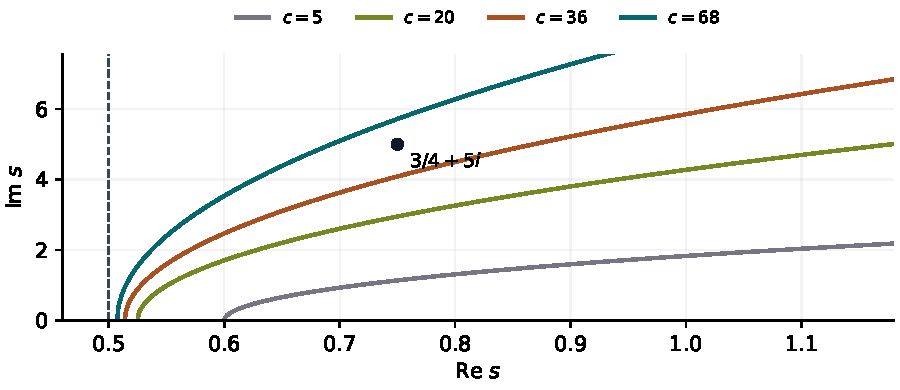
\includegraphics[width=.84\linewidth]{figures/disk_cover.pdf}\\[-1pt]
{\small Upper boundaries of four scheduled disks near the critical line. For each center, the portion below its curve and to the right of its left endpoint is inside the disk.}
\end{center}

\newpage\section{Liouville sums and convolution along perfect powers}\label{sec:powerdivisor}
The Möbius function vanishes at every multiple of a prime square. The Liouville function
$\lambda(n)=(-1)^{\Omega(n)}$ takes a nonzero sign at every positive integer, where
$\Omega(n)$ counts prime factors with multiplicity. Despite this difference, either sequence gives the same constructive square-root cancellation criterion, including uniform cancellation in reduced residue classes. An entire family of such replacements works with one growth witness.

\paragraph{The four input families.}
For RH use $a(n)=\mu(n)$. For progression GRH use the same coefficients and restrict sums to $n\equiv b\pmod q$, with $q\ge1$, $0\le b<q$, $(q,b)=1$. For cyclotomic GRH and Dedekind ERH use the signed reciprocal coefficients $a_F(n)$ described in Section~\ref{sec:matrices}, with $F=X^m-1$ and arbitrary monic $F$ of positive degree, respectively. We write $A(N)$ for the corresponding prefix and $A(0)=0$. Its growth statement requests, for every $r\ge1$, an integer $c$ with
\[
             |A(N)|^{2r}\le c N^{r+1}\quad(N\ge0).
\]
The progression constant precedes $q,b$. For the polynomial families the polynomial precedes the constant.

\begin{theorem}\label{thm:powerdivisor}
Fix any $h\ge2$. Replace $a$ everywhere by the integers
\[
   b_h(n)=\sum_{d^h\mid n}a(n/d^h)\qquad(n\ge1),
\]
and denote their corresponding prefixes by $B_h$. For each of the four families the growth statement is equivalent to the statement for $B_h$. It is also equivalent to the single sentence in which the same output constant works for every $h\ge2$. Both witness transformations take the input witness $c$ at $2r$ to
\[
                       C_r(c)=(c+1)(8r)^{2r}
\]
at $r$. This includes uniformity over all reduced progressions when that row is used.
\end{theorem}

\begin{proof}
First ignore residue conditions. At a finite cutoff, collecting the pairs $(d,m)$ with $d^h m\le N$ gives
\[
 B_h(N)=\sum_{d=1}^N A(\lfloor N/d^h\rfloor),\qquad
 A(N)=\sum_{d=1}^N \mu(d)B_h(\lfloor N/d^h\rfloor).
\]
For the second identity, substitute the first into the right side, use
$\lfloor\lfloor N/d^h\rfloor/e^h\rfloor=\lfloor N/(de)^h\rfloor$, and group pairs by $s=de$.
The coefficient of $A(\lfloor N/s^h\rfloor)$ is
$\sum_{d\mid s}\mu(d)=[s=1]$. Indeed the squarefree divisors are the subsets of the distinct prime factors, and for $s>1$ toggling its least prime factor pairs opposite signs. Terms with $s^h>N$ vanish. This proves finite inversion.

For residues, a summand $d^h m\equiv b\pmod q$ with reduced $b$ forces $(d,q)=1$.
For such $d$, find the unique representative $b_d$ with
$d^h b_d\equiv b\pmod q$ by testing the residues $0,\ldots,q-1$. Multiplication by $d^h$ is a permutation, and $b_d$ is again reduced. For $q=1$ the representative is always zero.
The forward formula now uses $A_{q,b_d}$ at its $d$th term and skips the nonunits. The reverse formula uses $\mu(d)B_{h,q,b_d}$. To verify inversion, a product $s=de$ is a unit exactly when both factors are units, and the residue selected in two steps is $b_s$. Thus every surviving coefficient reduces to the same divisor sum as before. In both directions the input bound applies to the index chosen at each term because its constant precedes all residue choices.

It remains to bound either signed sum. Write its $d$th term as $t_d$, set
$m_d=\lfloor N/d^h\rfloor$ and use $t_d=0$ at an excluded residue.
Since the kernel has absolute value at most one, the bound at $2r$ gives
$|t_d|^{4r}\le c m_d^{2r+1}$. For $N\ge1$ put $X=\max_{1\le d\le N} d|t_d|$.
As $d^2m_d\le N$,
\[
   (d|t_d|)^{4r}
   \le c d^{4r}m_d^{2r+1}
   \le c(d^2m_d)^{2r+1}
   \le c N^{2r+1}.
\]
It follows that $X^{4r}\le cN^{2r+1}$. The sum of the absolute values up to $2^j$ is at most $(j+1)X$, extending the sequence by zeros past $N$. Indeed the first term is bounded by $X$. In each subsequent block $2^j<d\le2^{j+1}$, every term satisfies $2^j|t_d|\le X$ and there are $2^j$ terms. Add those inequalities and cancel the positive factor $2^j$. If $\ell=\lfloor\log_2 N\rfloor$, this gives $|\sum t_d|\le (\ell+2)X$.

For every $k\ge1$, write $\ell=kz+s$ with $s<k$. Since $z+1\le2^z$, we have $\ell+2\le2k(z+1)\le2k\,2^z$. Raising to the $k$th power and using $kz\le\ell$ yields
\[
                       (\ell+2)^k\le (2k)^k N.
\]
Taking $k=4r$ therefore bounds $|\sum t_d|^{4r}$ by $c(8r)^{4r}N^{2r+2}$. Comparison with the square of $C_r(c)N^{r+1}$ proves the assertion. The empty cutoff is immediate. The same $C_r(c)$ works for every $h$. Conversely a uniform-power hypothesis can be specialized to $h=2$ before applying inversion.

All sums, maxima, quotient tests, parity calculations and powers in these arguments are primitive recursive. An invariant asserting a bound for every index below a finite cutoff can be expressed as the equality of a bounded-product test to one. Reindexing the double sums uses finite pairs and a bounded sum over each product fiber. The prime-factor toggling proof uses the least prime divisor found by bounded search. These arguments give quantifier-free induction proofs with the displayed parameters, followed by intuitionistic introduction and elimination of the outer quantifiers.
\end{proof}

\paragraph{What is being counted.}
For the rational coefficient, factor the divisor sum at a prime $p^e$. The only surviving quotients have $p$-adic exponent 0 or 1. Consequently
\[
 b_h(p^e)=
 \begin{cases}
  +1 & e\equiv0\pmod h,\\
  -1 & e\equiv1\pmod h,\\
  0 & \text{otherwise}.
 \end{cases}
\]
Distinct prime powers contribute independently. For $h=2$ these factors multiply to $(-1)^{\Omega(n)}$. For $h=3$ the coefficient at $4$ vanishes, at $8$ it is $+1$, and at $16$ it is $-1$. At cutoff $10$, $M(10)=-1$ whereas $\sum_{n\le 10}\lambda(n)=0$; the square-divisor identity reads $M(10)+M(2)+M(1)=0$. The reduced classes $1,2$ modulo $3$ give Liouville prefixes $2,-3$ respectively at the same cutoff.
For a polynomial $F$, the local coefficient sequence arises from
$U_{F,p}(T)/(1-T^h)$, with $U_{F,p}$ as in Appendix~\ref{sec:dedekind}. This formula retains every exceptional local factor used by the arithmetic input. It follows by multiplying a polynomial by the formal series $1+T^h+T^{2h}+\cdots$ and needs only the terms through the tested exponent.

\paragraph{Lean coverage.}
\code{PowerDivisorSyntax.statement} constructs the closed ProveIt formulas. The option \code{some j} fixes $h=j+2$ and \code{none} places $h$ after the constant. The optional direct implementation uses the prime-exponent rule for the rational and progression rows.
The lemma \code{power_divisor_transfer} proves the numerical estimate with arbitrary signed terms and cutoffs. The lemma \code{act_mul} checks the finite divisor regrouping for arbitrary integer arithmetic functions.
\code{growth_iff} and \code{uniform_growth_iff} prove both directions for every integer sequence $A$ with $A(0)=0$ on the unmasked prefixes, using Mathlib's Möbius function and its convolution identity. The theorem \code{mertens_iff_liouville} checks the equivalence for Mathlib's actual Möbius and Liouville sums. Its proof groups the lattice pairs $d^2m=n$ and shows by uniqueness of prime valuations modulo two that exactly one quotient is squarefree. The computation \code{check_power_divisors.py} independently compares the direct local factors and both progression transforms at $0\le N\le64$, $1\le q\le9$ and $2\le h\le6$. The residue transport and the identification of the compiled coefficient programs with these sums are proved above on paper. These analytic interpretations inherit the classical bridges for the respective Mertens families.

\section{One finite cube for all parameters}\label{sec:unary-cube}

How many inputs does a counterexample require? A Dedekind packet uses
five naturals, of which four specify a polynomial. One natural already
suffices to exhibit a failure, even if its only interpretation is a
common search radius. The conversion in both directions has explicit
primitive recursive witnesses. The same construction applies to the
Dirichlet and ordinary packets.

Write \(e(\mathbf x)\) for the truncated excess in the relevant
packet. For RH the free coordinate is \(t\), for GRH the coordinates
are \((d_0,t)\), and for ERH they are \((d_0,H,u,v,t)\).
Define \(B_e(N)\) by scanning every tuple in
\(\{0,\ldots,N-1\}^r\), starting with zero and setting the flag to
one on a nonzero sample. If \(N=0\), the flag is zero for all three
families. For instance, \(B_e(2)\) checks the 32 combinations of
coordinates zero and one for ERH, including both polynomial words
in each combination. For GRH it checks four combinations. The cost
can be enormous because the underlying excess itself performs large
integer computations. The interest here lies in the arity and
logical strength of the test.

\begin{theorem}\label{thm:cubef}
Let \(A=\forall x_1\cdots\forall x_r\,[e(\mathbf x)=0]\), allowing
an arbitrary iPRA term and additional free parameters in \(e\).
The following are equivalent by derivations of object iPRA:
\[
 A,\qquad \forall N\ B_e(N)=0,\qquad
 \forall N\ B_e\bigl(N+g(N)\bigr)=0
\]
for each given unary primitive recursive program \(g\). In addition,
object iPRA proves the witness-preserving equivalence
\[
 \bigl(\exists\mathbf x\ e(\mathbf x)\ne0\bigr)
 \quad\longleftrightarrow\quad
 \bigl(\exists N\ B_e(N)\ne0\bigr).
\]
For a block of length zero the construction uses the term itself in
place of a flag.
\end{theorem}

\begin{proof}
The proof concerns formal derivations, so the induction formulas matter.
For a row of samples \(f(j,\mathbf p)\), define its scan by
\[
 S(0,\mathbf p)=0,\qquad
 S(j+1,\mathbf p)=
 \begin{cases}
    S(j,\mathbf p),&f(j,\mathbf p)=0,\\
    1,&f(j,\mathbf p)\ne0 .
 \end{cases}
\]
The conditional is a PR symbol with its two branches proved from the
recursion equations. The object theory proves
\(S(j+1)=0\leftrightarrow(f(j)=0\land S(j)=0)\):
induct on the sampled value in the quantifier-free formula for the
conditional. If all samples vanish, induct on the atomic formula
\(S(j)=0\) to obtain every clean prefix. Conversely, fix arbitrary
\(x\) and induct on the slack \(d\) in the quantifier-free implication
\[
 S\bigl(d+(x+1)\bigr)=0\ \longrightarrow\ f(x)=0 .
\]
At zero use the current-sample conjunct of the successor law.
At the successor use the previous-prefix conjunct and the induction
hypothesis. These are first-order derivations with all remaining
parameters free.

Compile a scoped term to a PR symbol by mapping each variable to a
projection and each application to composition. Structural recursion on
the finite term gives a formal proof of the compiler's defining
equality. At a leaf the cube code evaluates this term. At a universal
binder, apply the row scan to the child's cube code, keeping the same
horizon \(N\) inside each child and scanning the new coordinate only
up to \(N\). A permutation and a duplication of arguments implement
this convention with PR composition. This recursion runs over fixed
syntax while constructing the derivation. The only arithmetic
inductions within iPRA are quantifier-free.

For the forward direction, open the universal binder, prove the child
cube clean and use the row-scan result. For the converse take an
arbitrary tuple \(\mathbf x\). Choose
\[
                   N_{\mathbf x}=\sum_{i=1}^r(x_i+1).
\]
For each coordinate the sum of the other summands is an explicit
slack \(d_i\) satisfying \(N_{\mathbf x}=d_i+(x_i+1)\).
The same equations hold at horizon \(N_{\mathbf x}+g(N_{\mathbf x})\)
after increasing each slack by \(g(N_{\mathbf x})\).
The needed laws of addition have quantifier-free induction proofs.
Apply the single-row reading implication once per binder and conclude
\(e(\mathbf x)=0\). This covers every finite tuple with one and the
same horizon. Choosing the horizon after introducing the tuple
preserves the order of the object quantifiers. In particular, a known
bad tuple gives a bad cube of radius \(N_{\mathbf x}\).

For the converse on positive failures, one additional primitive
recursion keeps an index \(I\), initially zero. At stage \(j+1\),
retain \(I(j)\) if \(f(j)=0\), and set it to \(j\) otherwise.
The correctness invariant is the quantifier-free formula
\[
                 S(j)\ne0\ \longrightarrow\ f(I(j))\ne0 .
\]
At a zero sample any dirty flag comes from the preceding step.
At a nonzero sample the stored index points to the present failure.
Zero tests are decidable in iPRA, so the two branches suffice.
Starting with a bad cube, read this index in its outer scan. The child
cube at that index is bad. Repeat through the finite syntax down
to the nonzero excess. In each nonempty scan the hit is its last
failing index. This constructs the existential tuple directly.
\end{proof}

For example \(g(N)=N^2\) tests only sizes \(N^2+N\) and
\(g(N)=2^N\) tests only \(N+2^N\). Neither schedule has to enumerate
all sizes. Its explicit slack makes it cofinal in a way that iPRA can
use. The uniform Lean results are \texttt{CubeTests.diagonal\_iff},
\texttt{CubeTests.schedule\_iff}, and \texttt{CubeTests.failure\_iff}.
The specializations \texttt{rh\_cube}, \texttt{grh\_cube} and
\texttt{erh\_cube} have the original closed packet statements on their
left sides.

\paragraph{The first radius of failure.}
One may also count the number \(C(m)\) of dirty cubes with radius
strictly below \(m\). A counterexample to an entire family is
equivalent, with witnesses in both directions, to
\[
              \exists m\,[C(m)=0\ \land\ B_e(m)\ne0].
\]
Indeed a bad tuple supplies a dirty radius, and bounded search up to
that radius finds its first dirty cube. Its hit selectors then recover
a bad tuple in that cube. Here the minimum is taken across all field
codes and cutoffs at once. At the first dirty radius \(m\), every
bad tuple in that cube has some coordinate equal to \(m-1\), since its
predecessor cube is clean. In particular this witness minimizes
\(1+\max_i x_i\) across counterexamples. For the three nonempty blocks
the zero-radius cube is empty.

The Lean proof \texttt{failure\_iff\_first\_radius} composes
the positive equivalence above with the supplied one-dimensional
first-failure extractor. The companion \texttt{census\_iff}
transports that archive's full catalogue of tests to \(C\). For
example, each of \(\forall m\, C(m+1)=C(m)\) and
\(\forall m\,\exists d\, C(m+1+d)=0\) is an object-theoretically
equivalent formulation for each family.


\newpage\section{Symmetric tests on a whole prefix}\label{sec:symmetric-prefixes}
Fix the polynomial parameters and abbreviate the archive's squared dyadic discrepancy and its allowance by
\[
 a_i=\bigl(B_F(2(i+100))-2B_F(i+100)\bigr)^2,\qquad
 b_i=(i+100)W_i^2,\qquad e_i=a_i\mathbin{\dot-}b_i .
\]
Here $B_F(y)=\lfloor\log_2 A_F(y)\rfloor$ and $W_i$ is the allowance at $i+100$. Thus the local hypothesis is $\forall i\;a_i\le b_i$. The following finite theorem applies to arbitrary natural data. Its tests are invariant under simultaneous permutation of the pairs $(a_i,b_i)$ in the prefix.

\begin{theorem}\label{thm:symmetric-prefix}
Fix a horizon $m\ge0$. Define
\[
 h=1+\sum_{i<m} b_i,\qquad z_i=a_i+(h-b_i)\quad(i<m),
 \qquad r=mh+1,\qquad U=\sum_{i<m}a_i.
\]
Each of the following tests is equivalent to $a_i\le b_i$ for every $i<m$:
\begin{align}
 \sum_{i<m} z_i^{\,r}&\le m h^r, \label{eq:sym-mom}\\
 \sum_{i<m}(m+1)^{z_i}&\le m(m+1)^h, \label{eq:sym-exp}\\
 \prod_{s=1}^{U}\,\prod_{i<m}\left|s+b_i-a_i\right|&>0 .
 \label{eq:sym-char}
\end{align}
In particular each test detects every failure by the first horizon containing it.
\end{theorem}
\begin{proof}
Since $b_i\le h$, the subtraction in $z_i$ is exact. Thus $z_i\le h$ is equivalent to $a_i\le b_i$. This proves the forward directions of \eqref{eq:sym-mom} and \eqref{eq:sym-exp} by addition of $m$ bounds. The challenge with the converse is that many small terms can mask a single violation.

For positive $h$ and every $j\ge0$,
\[
 (h+1+j)h^j\le(h+1)^{j+1}.
\]
At $j=0$ this is equality. Multiplying the lower bound at $j$ by $h+1$ produces the desired lower bound at $j+1$ plus $(j+1)h^j$. Take $j=mh$. Because $h^j>0$ and $mh<h+1+mh$, we obtain
\[
 m h^{mh+1}=(mh)h^{mh}<(h+1+mh)h^{mh}\le(h+1)^{mh+1}.
\]
If $a_i>b_i$, its single term $z_i^r$ already exceeds the entire allowance $mh^r$. The exponential test has the same implication with a shorter calculation: $(m+1)^{h+1}>m(m+1)^h$. Both directions use comparisons of natural numbers only.

For the product test, $a_i\le b_i$ makes every factor at least $s\ge1$. If $a_i>b_i$, its positive difference $s=a_i-b_i$ satisfies $1\le s\le a_i\le U$ and gives a zero factor. This also explains the upper end of the product. At $m=0$ both sums vanish and the product is $1$. If $U=0$, every $a_i$ vanishes.
\end{proof}

\paragraph{Polynomial interpretation.}
The inner product in \eqref{eq:sym-char} equals $|P_m(s)|$ for the split monic integer polynomial
\[
 P_m(X)=\prod_{i<m}(X+b_i-a_i).
\]
The test excludes every positive integer root. Two other finite descriptions are $P_m(s)>0$ for every $1\le s\le U$ and nonnegativity of every coefficient of $P_m$. When all $b_i-a_i$ are nonnegative each factor has nonnegative coefficients and positive value on those integers. Conversely, a violation gives a positive root in the tested interval, and a monic polynomial with nonnegative coefficients has strictly positive value there, since its leading term is already positive. The coefficient test is PR: starting with $1$, multiply the current coefficient vector by $X+b_i-a_i$, using signed pairs of naturals. The absolute-value product has a checked PR matrix. In \texttt{CoefficientTest.lean} the leading coefficient $1$ is implicit and the lower coefficients form a finite list in ascending order. Horner evaluation and multiplication by $X+b_i-a_i$ obey the polynomial identities by list induction. The theorems \texttt{grid\_iff} and \texttt{coefficients\_iff} check the signed-grid and coefficient equivalences for every finite horizon in ordinary Lean arithmetic. Both readings inherit the same three family closures.

\paragraph{Example of the amplification.}
For $(a_0,a_1)=(4,0)$ and $(b_0,b_1)=(3,5)$ the sum of the two $a_i$ falls below the sum of the two $b_i$, despite the first violation. At $m=2$ the translated levels are $10$ and $4$, against $h=9$. The integer exponent $19$ makes $10^{19}>2\cdot9^{19}$. The exponential test already fails from $3^{10}>2\cdot3^9$, and the polynomial $(X-1)(X+5)$ vanishes at $s=1$.

\paragraph{A multiplicative certificate with an object derivation.}
Use the actual nonnegative excess $e_i$ to form $V(0)=1$ and
$V(m+1)=V(m)(1+e_m)$. Then the hypothesis has the equivalent form
\[
                    \forall m\quad V(m)=1.
\]
This is also the determinant of the diagonal matrix with entries $1+e_i$ being $1$ at every horizon. If all $e_i$ vanish, quantifier-free induction on the equality $V(m)=1$ gives the assertion. In the converse, instantiate it at $m$ and $m+1$. The recursion yields $1+e_m=1$ and successor injectivity gives $e_m=0$. This reasoning avoids factoring an integer product in the object theory. The compiled code builds the multiplication step from the same PR symbols as the original packet. The Lean theorems \texttt{rh\_iff}, \texttt{grh\_iff} and \texttt{erh\_iff} in \texttt{RiemannIPRA.ProductCertificate} are empty-context derivations of the corresponding biconditionals in \texttt{Prf PRAAx}.

\paragraph{Quantifiers and proof strength.}
In Theorem~\ref{thm:symmetric-prefix}, take all $m$. For the converse choose $m=i+1$ at a desired index $i$. Ordinary RH fixes $(d_0,H,u,v)=(0,0,0,1)$, Dirichlet GRH varies $d_0$ in $(d_0,0,0,1)$, and Dedekind ERH varies all four parameters. The three tests therefore give nine closed $\Pi^0_1$ sentences. The exponents, sums, products and both bounds on the polynomial grid are all primitive recursive. In iPRA, bounded universal predicates here can be written as a product of their $0$--$1$ truth values. A single summand is at most the partial sum containing it, by induction on the prefix length with its index free. A sum over an initial interval with all summands $\le c$ is $\le mc$ by accumulating this bound, and a product is positive precisely when each factor is positive by the product recursion. For guard-dependent applications, replace the finite conjunction by its recursively updated truth bit and induct on the implication from that bit to the accumulator bound. These are quantifier-free inductions. The power comparisons use the same induction on integers displayed above. The algorithm for recovering an offending index, when one of the three finite tests fails, is the bounded scan for the first $a_i>b_i$. This never uses an unbounded search.

\texttt{SymmetricPrefixes.lean} proves the finite equivalences, the reading of each compiled PR matrix, and \texttt{statement\_iff} for the standard-natural denotations of the closed sentences. The argument above gives the iPRA arithmetic proof; its translation to a \texttt{Prf} term is provided for the multiplicative certificate. The passage from these arithmetic criteria to the respective statements about analytic zeros uses the same external correspondence as the original prime-product sentence.

\newpage\section{Constructing the primitive-recursive term}\label{sec:kernel}
The repository's \code{PR k} is syntax for a function of arity \(k\). Its constructors are zero, successor, projection, composition and primitive recursion. The last takes a base \(f(\vec x)\) and a step \(g(j,a,\vec x)\), and feeds the previous value into \(a\). A term applies such a fixed tree to scoped variables or other terms. The repository's \code{Fm} supplies implication and both number quantifiers, and \code{PRAAx} admits induction for quantifier-free formulas \cite{repo}.

\paragraph{Bounded operations.}
An aggregate over \(j<N\) starts from its neutral value and updates an accumulator for each \(j\). Addition, multiplication, maximum, existential and universal bit tests have this form, including the empty range. In the step the counter is at index 0, the accumulator is at 1 and each old parameter moves up two places. \code{PacketLanguage.program} performs this translation at arbitrary arity. The theorem \code{value_program} proves by induction on the source expression that its PR tree evaluates to the direct bounded-fold semantics for every assignment. Evaluation of an arbitrary syntax tree is in the Lean metatheory. The object language uses only the fixed tree for \(E\).

Truncated subtraction iterates predecessor. For \(b>0\) the quotient of \(a\) by \(b\) is the largest \(i\le a\) satisfying \(ib\le a\). The remainder is \(a-b\lfloor a/b\rfloor\). A maximum up to \(y\) computes the largest \(i\) with \(2^i\le y\) for positive \(y\). Primality tests all proposed divisors \(2,\ldots,p-1\) after testing \(p\ge2\). Thus all loops have natural-number bounds supplied by previously constructed PR functions.

\paragraph{Finite-field calculation.}
In \(\F_p[X]\), \(X^{p^k}-X\) has each monic irreducible factor of degree dividing \(k\) exactly once. Indeed its roots are precisely the elements of \(\F_{p^k}\). A degree-\(e\) root has Frobenius orbit of length \(e\), and the derivative is \(-1\). Hence \eqref{eq:h} sums \(e\) over the distinct degree-\(e\) irreducible divisors of \(\bar F\) with \(e\mid k\). A monic degree-\(e\) candidate has exactly \(p^e\) possible lower coefficient words. Divisibility by it is tested by comparing coefficients against all \(p^{d-e}\) monic quotients. A degree-\(e\) candidate is irreducible precisely when the search finds no monic divisor of degree \(1,\ldots,e-1\). Each factor is visited once, even when repeated in \(\bar F\). Digits of the two input words are reduced by computing \((a+p-(b'\bmod p))\bmod p\). The inner subtraction has no truncation loss.

\paragraph{Finishing the matrix.}
For \(p\le y\), take \(1\le k\le\lfloor\log_2 y\rfloor\), multiplying by \(p^{h_F(p,k)}\) only for primes with \(p^k\le y\). This exhausts the product since \(p\ge2\). Compute absolute difference by \((a\mathbin{\dot-}b)+(b\mathbin{\dot-}a)\), square and compare. These instructions define \code{RiemannIPRA.excess : PR 5} without analytic parameters. The Python evaluator uses Euclidean gcd and modular powering to compute the same integer more quickly.
\newpage
\section{What the polynomial counts at a prime}\label{sec:local}
Write \(F=\prod_{i=1}^r f_i^{a_i}\) over \(\Q\), with the \(f_i\) distinct monic irreducibles, and set \(G=\prod_i f_i\), \(K_i=\Q[X]/(f_i)\). By Gauss's lemma all these polynomials have integral coefficients. Two different \(f_i\) may give isomorphic fields. Each contributes a summand. Define
\[
 \Psi_F(y)=\log A_F(\lfloor y\rfloor)
   =\sum_{p^k\le y}h_F(p,k)\log p,\qquad
 \psi_K(y)=\sum_{N\mathfrak p^a\le y}\log N\mathfrak p ,
\]
where the second sum ranges over prime ideals and \(a\ge1\). Here and below an undecorated \(\log\) is natural. Let \(D=|\disc(G)|\), with \(D=1\) in degree one.

\begin{lemma}\label{lem:exception}
For \(p\nmid D\), the coefficient of \(\log p\) at \(p^k\) in \(\sum_i\psi_{K_i}\) is \(h_F(p,k)\). For every \(y\ge2\),
\[
 \left|\Psi_F(y)-\sum_i\psi_{K_i}(y)\right|\le d\,\omega(D)\log y,\quad
 \sum_i\log|\Delta_{K_i}|\le\log D\le 2d^2(H+2),
\]
where \(\omega(D)\) counts distinct rational prime divisors and \(\Delta_K\) is the field discriminant.
\end{lemma}
\begin{proof}
The discriminant of \(G\) is the product of the discriminants of its factors times the squares of their pairwise resultants. For \(\alpha_i=X\bmod f_i\), the discriminant of \(f_i\) is \(\Delta_{K_i}[\mathcal O_{K_i}:\Z[\alpha_i]]^2\). Away from \(D\) all these indices are units modulo \(p\), the factors remain pairwise coprime, and the quotients \(\mathcal O_{K_i}/p\mathcal O_{K_i}\) and \(\F_p[X]/\bar f_i\) coincide. Decomposing the latter into finite fields identifies the degrees of its irreducible factors with the residue degrees \(e_{\mathfrak p}=[\mathcal O_{K_i}/\mathfrak p:\F_p]\). Each prime ideal with \(e_{\mathfrak p}\mid k\) contributes \(e_{\mathfrak p}\log p\) at \(p^k\). This gives the claimed coefficient by \eqref{eq:h}.

At every prime the sum of the residue degrees above \(p\) is at most \([K_i:\Q]\), since the ramification indices are positive. Both competing coefficients at \(p^k\), measured in units of \(\log p\), lie between \(0\) and \(d\). At one exceptional prime their total discrepancy is at most \(d\lfloor \log y/\log p\rfloor\log p\). This proves the first inequality. The discriminant product gives \(\prod_i|\Delta_{K_i}|\le D\).

Put \(R=H+2\). All lower coefficients of \(F\) have absolute value at most \(R-1\). For \(|z|>R\), the leading term exceeds the sum of the absolute values of the lower terms by the geometric series bound. All roots of \(G\) therefore have absolute value at most \(R\). The pairwise-differences formula gives \(D\le(2R)^{d(d-1)}\), including \(d=1\). Taking logarithms and using \(\log(2R)\le2R\) finishes the proof.
\end{proof}
Using \(G\) in this proof matters. The discriminant of \(F\) can vanish when \(F\) has a repeated factor. Neither \(G\) nor \(D\) needs to be computed by the test.
\newpage
\section{Why zeros on the critical line imply every test}\label{sec:forward}
\begin{proposition}\label{prop:forward}
Fix a code for \(F\). If the critical-strip zeros of each \(\zeta_{K_i}\) have real part \(1/2\), its arithmetic matrix holds for every \(n\ge100\).
\end{proposition}
\begin{proof}
We use the fieldwise explicit prime ideal theorem of Greni\'e and Molteni \cite[Corollary 1.2]{gm}. For \(y\ge100\), under the Riemann hypothesis for \(\zeta_K\), it gives
\begin{equation}\label{eq:gm}
|\psi_K(y)-y|\le \sqrt y\left[
 \left(\frac{\log y}{2\pi}+2\right)\log|\Delta_K|
 +\left(\frac{(\log y)^2}{8\pi}+2\right)[K:\Q]\right].
\end{equation}
For integer \(y\ge100\), \(\log y\le L(y)\). Each multiplier in parentheses is at most \(3L(y)^2\). Write \(S=\sum_i\log|\Delta_{K_i}|\). Summing \eqref{eq:gm} gives \(3\sqrt y L(y)^2(S+d)\). By Lemma~\ref{lem:exception}, \(S+d\le3d^2R\). The extra error at bad primes is at most
\[
 d\,\omega(D)\log y\le 2d\log D\log y\le 4d^3R\log y,
\]
using \(2^{\omega(D)}\le D\) and \(1/\log 2<2\). Combining the two estimates yields
\begin{equation}\label{eq:rough}
             |\Psi_F(y)-ry|\le 13d^3R\sqrt y\,L(y)^2 .
\end{equation}
In particular the unknown rational factor count \(r\) cancels in
\(\Psi_F(2n)-2\Psi_F(n)\). Since \(B_F(y)=\lfloor\Psi_F(y)/\log 2\rfloor\), taking integer parts adds at most \(3\) to the absolute dyadic error after division by \(\log 2\). Equation~\eqref{eq:rough} at \(n,2n\) now gives
\[
 |D_n|\le 3+
 \frac{13(\sqrt2+2)}{\log2}\, d^3R\sqrt n L(2n)^2
 \le 110d^3R\sqrt n L(2n)^2 .
\]
The chosen constant \(C(d,H)\) dominates \(110d^3R\) for every allowed code. Squaring proves \(D_n^2\le nW^2\).
\end{proof}

\paragraph{Why a loose constant can still imply RH.}
For each fixed polynomial the constant is independent of \(n\). A zero at \(s=\rho\) with \(1/2<\Re\rho<1\) forces a singularity of a transform of this dyadic difference. A bound \(O_F(\sqrt n\log^2 n)\), however large its fixed coefficient, makes that transform holomorphic throughout \(\Re s>1/2\). The multiplier in the transform explains why subtracting the values at \(n\) and \(2n\) preserves every off-line obstruction in the critical strip.
\newpage
\section{Recovering zero-freeness from the integer inequality}\label{sec:reverse}
\begin{proposition}\label{prop:reverse}
Fix one code for \(F\). If its test holds for all \(n\ge100\), every zero of every \(\zeta_{K_i}\) in \(0<\Re s<1\) lies on the critical line.
\end{proposition}
\begin{proof}
Set \(V(x)=\Psi_F(2x)-2\Psi_F(x)\) for real \(x\ge1\), using right-continuous step functions. At an integer \(n\ge100\), restoring the discarded fractions gives
\(|V(n)|\le(\log2)(C(d,H)\sqrt n L(2n)^2+3)\).
For \(n=\lfloor x\rfloor\), \(\Psi_F(x)=\Psi_F(n)\) and the interval \((2n,2x]\) contains at most one integer. Its jump is at most \(d\log(2n+1)\), since an integer is a positive power of at most one prime. Thus
\[
  V(x)=O_F\!\left(\sqrt{x}(1+\log x)^2\right),\qquad x\ge1.
\]
On the finite interval below 100 the step function is bounded. Consequently
\[
  T(s)=s\int_1^\infty V(x)x^{-s-1}\,dx
\]
is holomorphic on \(\Re s>1/2\). On compact subsets the integrand and its derivatives are dominated by an integrable power times a fixed power of \(\log x\).

On \(\Re s>1\), put \(J_F(s)=\sum_{p,k}h_F(p,k)(\log p)p^{-ks}\). The coefficients at integers are bounded by \(d\log n\), so termwise integration of the step function is justified by absolute convergence and gives \(J_F(s)=s\int_1^\infty\Psi_F(x)x^{-s-1}\,dx\). Substituting \(y=2x\) in the first term of \(T\), and using \(\Psi_F=0\) on \([1,2)\), gives
\begin{equation}\label{eq:mellin}
 T(s)=(2^s-2)J_F(s),\qquad
 J_F(s)=-\sum_i\frac{\zeta'_{K_i}(s)}{\zeta_{K_i}(s)}+U_F(s).
\end{equation}
The second equality follows by logarithmically differentiating the Euler products and using Lemma~\ref{lem:exception}. The correction \(U_F\) is a sum over the finite set \(p\mid D\) of power series in \(p^{-s}\) with coefficients of modulus at most \(d\log p\). It is holomorphic on \(\Re s>0\).

Use meromorphic continuation of the field zeta functions and the identity theorem to extend the right side of \eqref{eq:mellin} in its multiplied form to \(\Re s>1/2\). At a zero \(\rho\) with \(1/2<\Re\rho<1\), each vanishing zeta factor contributes minus its multiplicity to the residue of \(J_F\). Their sum is nonzero because the only field zeta pole is at 1. Also \(2^\rho-2\ne0\), since \(|2^\rho|=2^{\Re\rho}<2\). This contradicts holomorphy of \(T\). Finally, the functional equation of the completed Dedekind zeta function reflects nontrivial zeros across the critical line. Its gamma factors are regular and nonzero in the open strip \cite[eq.~(2.3)]{gm}. A zero to the left would therefore give one to the right.
\end{proof}
The transform multiplier has zeros on \(\Re s=1\). The hypotheses concern the open critical strip. Nonvanishing on its boundary at \(\Re s=1\) is a separate classical theorem.
\newpage
\section{Identifying the three analytic families}\label{sec:families}
\begin{theorem}\label{thm:main}
In the classical standard model of arithmetic the three sentences of Section~\ref{sec:sentence} are respectively equivalent to RH, Dirichlet GRH and Dedekind ERH.
\end{theorem}
\begin{proof}
\emph{Riemann.} \(X-1\) gives the single field \(\Q\), whose Dedekind zeta is the ordinary Riemann zeta. Propositions~\ref{prop:forward} and \ref{prop:reverse} apply directly.

\emph{Dirichlet.} Over \(\Q\), \(X^m-1=\prod_{e\mid m}\Phi_e(X)\). Its distinct factors give the list of cyclotomic fields \(\Q(\zeta_e)\), with their occurrences as factors. For each \(e\), the cyclotomic factorization is
\[
 \zeta_{\Q(\zeta_e)}(s)
    =\prod_{\substack{\chi\text{ primitive}\\\operatorname{cond}(\chi)\mid e}} L(s,\chi).
\]
It uses the primitive characters of conductors dividing \(e\), including the conductor-one character \cite[Thm.~19.15]{suth}. In the open strip each factor is holomorphic, so zeros of a factor persist in the product. If Dirichlet GRH holds, all the field factors associated to every \(X^m-1\) satisfy the premise of Proposition~\ref{prop:forward}. Conversely, for a primitive character of conductor \(m\) choose that input \(X^m-1\). Proposition~\ref{prop:reverse} gives critical-line localization for \(\zeta_{\Q(\zeta_m)}\), hence for \(L(s,\chi)\). This includes complex characters and imposes no bound on the conductor. An imprimitive character merely inserts factors \(1-\chi^*(p)p^{-s}\), whose possible zeros have real part zero.

\emph{Dedekind.} Every \(K_i\) from an admissible input is a number field, giving the forward direction under ERH. Conversely, take any number field \(K\). In characteristic zero the primitive element theorem gives \(K=\Q(\alpha)\). Multiplying \(\alpha\) by an integer clearing the denominators of its monic rational equation makes it integral and leaves the generated field unchanged. Its monic minimal polynomial thus occurs in our coding. Proposition~\ref{prop:reverse} applies whether or not \(K\) is Galois.
\end{proof}

\paragraph{Quantifier scope and constructive content.}
An input is a finite tuple and failure is the decidable strict integer inequality \(D_n^2>nW^2\). The explicit bound eliminates the need to choose a growth constant for each field. An absolute ordering of all constructive versions would require a specified comparison language. The result here is classical equivalence for the entire analytic family, with an explicit universal, decidable test.

\paragraph{A contour variant.}
In ProveIt's \emph{zeta zero distribution} packet, a rational contour carries boundary clearance, a precision and a winding number \cite{zero}. A certified nonzero winding on a pole-free rectangle strictly inside one side of the strip would locate a counterexample for ordinary \(\zeta\). Classically an isolated off-line zero admits such a rectangle. A uniform constructive characterization requires proved enclosure, clearance and completeness results for the specified functions. That packet labels its Lean interface uncompiled. The integer sentences above are independent of those obligations.
\newpage
\section{The original Lean derivations}\label{sec:verified}
The project uses the ordinary iPRA interface in ProveIt at commit
\href{https://github.com/VladimirReshetnikov/ProveIt/tree/ce0e3ceaf41a83e653857e5f60e0460733cc230c/Logic/PrimitiveRecursiveArithmetic}{\code{ce0e3ceaf41a}}. Four unchanged modules define scoped syntax, deduction, PR functions and term models. The repository also has a transfer theorem to the native scalar calculus. Our checked derivations use its ordinary \code{PRAAx} calculus directly.
\begin{center}\small
\begin{tabular}{@{}p{.35\linewidth}p{.60\linewidth}@{}}\toprule
Lean declaration or file & Verified content\\\midrule
\code{PacketLanguage.value_program} & Compilation preserves bounded-expression values at every natural assignment.\\
\code{ArithmeticReading.lean} & Correct division, remainder, integer logarithm and primality tests.\\
\code{PolynomialCode.lean}, \code{Hypotheses.lean} & Actual PR trees for modular factor enumeration and the excess, then three closed formulas.\\
\code{rh_reading}, \code{grh_reading}, \code{erh_reading} & Standard-model interpretation gives the indicated universal tests in the specified argument order.\\
\code{naturalTerms_sound} & A derivation from hypotheses true in the standard model concludes a formula true there.\\
\code{erh_implies_grh}, \code{grh_implies_rh} & Closed \code{Prf PRAAx []} derivations of the two implications.\\
\code{erh_iff_no_counterexample} and its two specializations & Each universal zero-test is constructively equivalent to the negation of a finite failing tuple.\\\bottomrule
\end{tabular}
\end{center}
The last result uses a fact internal to iPRA. For any numerical term \(t\), one has \(t=0\lor\neg(t=0)\). Apply quantifier-free induction to \(z=0\lor\neg(z=0)\): at zero the left side holds by reflexivity, and at every successor the right side is a successor axiom. Hence \(\neg\neg(t=0)\Rightarrow t=0\). Through a universal prefix, intuitionistic quantifier introduction and elimination then derive
\[
  \forall\vec x\,E(\vec x)=0\quad\longleftrightarrow\quad
        \neg\exists\vec x\,\neg(E(\vec x)=0).
\]
Extracting a tuple from the negation of the whole universal assertion would be an additional logical step. The two hierarchy implications need only universal specialization and generalization.

The finite-field identification \eqref{eq:h}, the good-prime comparison, and the analytic equivalences in Theorem~\ref{thm:main} are justified by the mathematical proofs in this report. The Lean project contains no axiom asserting a Riemann hypothesis or those comparison theorems. Hypothesis formation and proofs of implications are distinct Lean judgments.
\newpage
\section{Exact examples for the prime-product test}
For the linear input \(X-1\), \(B_F(n)\) equals the binary length of \(\operatorname{lcm}(1,\ldots,n)\) minus one. For \(X^2+1\), at the rational prime 3 the polynomial stays irreducible. It contributes 0 to \(h_F(3,1)\) and 2 to \(h_F(3,2)\). At 2 its double root contributes only 1. At 5 its two linear factors contribute 2 for every \(k\ge1\). These cases check the handling of residue degrees, splitting and repeated roots.
\begin{center}\small
\begin{tabular}{@{}lrlrrr@{}}\toprule
Polynomial & \(n\) & \((d,H,u,v)\) & \(B_F(n)\) & \(B_F(2n)\) & \(D_n\)\\\midrule
\(X-1\) &100&\((1,0,0,1)\)&135&297&27\\
\(X^2+1\) &100&\((2,0,1,0)\)&135&299&29\\
\(X^3-2\) &100&\((3,1,0,2)\)&111&267&45\\
\(X^5-1\) &256&\((5,0,0,1)\)&732&1436&\(-28\)\\
\(\Phi_5\) &256&\((4,0,15,0)\)&377&701&\(-53\)\\\bottomrule
\end{tabular}
\end{center}
For the first row \(D_n^2=729\) and the right side of the inequality is \(1{,}677{,}721{,}600{,}000{,}000\). Large slack is expected at small \(n\). In the two final rows, \(X^5-1=(X-1)\Phi_5\). The test for the cyclotomic family uses the entire polynomial on the fourth row. The third row illustrates a non-Galois cubic field.

Run \code{python3 check_packets.py} for the independent finite-field, least-common-multiple and Gaussian splitting comparisons. To reproduce row four run \code{python3 check_packets.py 5 0 0 1 256}. All computations use integer arithmetic. In Lean, \code{SmokePR.lean} checks four local degrees, the binary logarithm of \(7\), and the smallest nonempty prime product. Its vector evaluator is proved equivalent to the interpreter for the original PR constructors. Repeated binary digit and bounded quotient searches make that literal evaluator expensive. The two algorithms agree by the finite-field argument of Section~\ref{sec:kernel}. A general machine-checked equivalence with the Python program is outside the formal results.

The archive is a Lake project pinned to Lean and Mathlib 4.32.0. The selective Mathlib cache command in \code{README.md} accelerates the first build. Running \code{lake build} checks the full default target. From a normal TeX installation, \code{latexmk -pdf report.tex} rebuilds the report. Exact dependency information and module names are in \code{README.md}.

\newpage\input{objectforms}
\input{slack}
\input{discreteforms}
\input{analyticforms}
\input{matrices}
\input{energy}
\input{farey-rh}
\input{series}
\input{lagarias}
\section{Verification and further research questions}\label{sec:buildnew}
The default Lake target imports the arithmetic syntax, the deep derivations and the finite number-theoretic proofs. The audit file \code{verification/Audit.lean} imports that target, displays representative theorem types, and prints their dependencies on Lean kernel axioms. The results are recorded in \code{verification/lean-audit.txt}. In particular:
\begin{itemize}\setlength\itemsep{2pt}
\item \code{CubeTests.failure_iff_first_radius} and the three cube biconditionals give actual derivations in the scoped object theory. A nonzero cube supplies a tuple without an appeal to Markov's principle or unbounded minimization.
\item \code{SplitPrimes.unary_grh_iff} proves the standard-natural equivalence of the bounded maximum and the unrestricted family. The cutoff beyond which an individual fixed field is eligible in the unary ERH test, and the analytic implications of complete splitting, are justified in Section~\ref{sec:split}.
\item \code{Taylor.statement_reading} interprets each compiled Taylor formula as the integer comparison of Section~\ref{sec:taylor}. The Cauchy bound and the converse through pole detection are mathematical proofs in that section.
\item \code{LiouvilleCriterion.mertens_iff_liouville} refers to the actual Mathlib functions. The theorem gives both directions of a growth-witness transformation; it does not assume any growth estimate.
\end{itemize}
When a theorem about \code{Prf PRAAx} uses function extensionality in Lean to identify substitutions, its object proof still uses only the rules of iPRA. Some ordinary Mathlib results depend on classical choice in their metatheory. Their types and the audit distinguish these from the construction of an internal derivation. The four Python checkers exercise finite computations independently.
\paragraph{Further research questions.}
Can the local modular splitting criterion $F\mid(X^p-X)^d$ be linked to the compiled irreducible-divisor search entirely within \code{Prf PRAAx}? Can one give a direct internal conversion between the prescribed prime envelope and a Mertens growth witness for the same field? Can the quantitative Taylor evaluation and center-translation identity be formalized over a first-order coding of local Cauchy names, using the explicit margins in Section~\ref{sec:taylor}?

\appendix\newpage
\section{Square-root cancellation as a second formulation}\label{sec:mertens-start}
A familiar alternative tests the summatory coefficients \(M(x)\) of reciprocal Euler products. For an integer \(z\) set
\[
    P(k,c,x,z)\quad\Longleftrightarrow\quad
     |z|^{2(k+1)}\le c\,x^{k+2}.
\]
The exponent on taking the \(2(k+1)\)-th root is \(1/2+1/(2(k+1))\). These exponents approach \(1/2\) from above. A bound for them gives a bound with any fixed positive slack. Conversely round the corresponding powered implied constant upwards. The sum at \(x=0\) vanishes. The file \code{MertensForms.lean} gives the following supplementary readings as constructive Lean propositions over naturals:
\begin{align*}
 &\forall k\,\exists c\,\forall x\ P(k,c,x,M(x)),\\
 &\forall k\,\exists c\,\forall q,a,x\
    ((q\ge1,\ 0\le a<q,\ (q,a)=1)\Rightarrow P(k,c,x,M_{q,a}(x))),\\
 &\forall f,k\,\exists c\,\forall x\ P(k,c,x,M_f(x)).
\end{align*}
Here \(M_{q,a}\) is a progression sum and \(f\) is the single-number polynomial code specified in Appendix~\ref{sec:dedekind}. These are witness formulations: for each supplied \(k\), the existential asks for a bound valid for all \(x\). The Dirichlet version places the constant before the modulus and the residue. The object sentences in Section~\ref{sec:sentence} instead supply the entire envelope in advance. The classical correspondences proved below do not identify the witness principles with the universal sentences inside iPRA.

\paragraph{A reciprocal-series estimate.}
We record the analytic detail needed for the all-fields witness formulation. Suppose \(Z(s)=\prod_{i=1}^r\zeta_{K_i}(s)\) has no zeros for \(\Re s>1/2\), with its pole at 1 understood. Let \(A(s)=U(s)/Z(s)=\sum a_n n^{-s}\) on \(\Re s>1\), where \(U\) is a finite product of powers of \(1-p^{-js}\), integer \(j>0\), and \(\sum |a_n|n^{-2}<\infty\). Then \(\sum_{n\le x}a_n=O_{Z,U,\epsilon}(x^{1/2+\epsilon})\) for every \(\epsilon>0\).

For details, fix \(1/2<b<1\). At large \(|t|\) take a disk centered at \(2+it\), of radius strictly between \(2-b\) and \(3/2\). A branch of \(\log Z\) agrees at its center with the Euler-product logarithm. The usual polynomial growth of fixed field zeta functions in fixed vertical strips bounds \(\Re\log Z=O(\log(2+|t|))\) on the disk. This growth also follows from their functional equations, Stirling's formula and the Phragm\'en--Lindel\"of principle using their classical finite order. On a slightly smaller disk with radius still larger than \(2-b\), Borel--Carath\'eodory bounds the absolute value of this logarithm by the same order. On radius \(1/2\) the Euler-product logarithm is bounded. Hadamard's three-circles theorem bounds \(|\log Z|\) on radius \(2-b\) by \(O((\log(2+|t|))^\theta)\) for a fixed \(\theta<1\). Therefore \(A(\sigma+it)\ll_{b,\eta}(1+|t|)^\eta\) for every \(\eta>0\), uniformly on \(b\le\sigma\le2\). Compact heights are covered by holomorphy of the reciprocal.

Take \(X=N+1/2\), \(T=X^4\). Truncated Perron's formula on \(\sigma=2\) has error \(O(X^3/T)\): the termwise truncation error is bounded by a constant times \((X/n)^2\min(1,1/(T|\log(X/n)|))\), and \(|\log(X/n)|\gg X^{-1}\) for every integer \(n\). Shift to \(\sigma=b\). The horizontal integrals cost \(O(X^2 T^{\eta-1})\), the vertical integral \(O_{b,\eta}(X^bT^\eta)\). Choosing \(b\) sufficiently close to \(1/2\) and then \(\eta>0\) sufficiently small proves the claim. Conversely a bound with every positive slack gives local uniform convergence of the reciprocal Dirichlet series by summation by parts, detailed for characters in Appendix~\ref{sec:dirichlet}.
\input{dirichlet}
\input{erh}
\begin{thebibliography}{10}\small
\bibitem{aramata} H. Aramata. \emph{\"Uber die Teilbarkeit der Dedekindschen Zetafunktionen}. Proc. Imp. Acad. 9 (1933), 31--34. \href{https://doi.org/10.3792/pia/1195580866}{Original paper}. See also R. Brauer, \emph{On the zeta-functions of algebraic number fields}, Amer. J. Math. 69 (1947), 243--250.
\bibitem{lagarias} J. C. Lagarias. \emph{An elementary problem equivalent to the Riemann hypothesis}. Amer. Math. Monthly 109 (2002), 534--543. Theorems 1.1, 3.1--3.2 and Lemma 3.2. \href{https://arxiv.org/abs/math/0008177}{Author's paper}.
\bibitem{wilf} H. S. Wilf. \emph{The Redheffer matrix of a partially ordered set}. Electron. J. Combin. 11 (2004), R10. \href{https://arxiv.org/abs/math/0408263}{Author's paper}.
\bibitem{repo} V. Reshetnikov and ProveIt contributors. \emph{Intuitionistic primitive recursive arithmetic}, ordinary ConciseIPRA syntax and calculus. \href{https://github.com/VladimirReshetnikov/ProveIt/tree/ce0e3ceaf41a83e653857e5f60e0460733cc230c/Logic/PrimitiveRecursiveArithmetic}{Pinned repository snapshot}.
\bibitem{zero} ProveIt. \emph{Zeta zero distribution in intuitionistic primitive recursive arithmetic}, especially the status section and \code{lean/ObjectTargets.lean}. \href{https://github.com/VladimirReshetnikov/ProveIt/tree/ce0e3ceaf41a83e653857e5f60e0460733cc230c/Logic/PrimitiveRecursiveArithmetic/docs/proofs/analytic-number-theory/zeta_zeros_ipra_2026-11-15}{Research packet}.
\bibitem{gm} L. Greni\'e and G. Molteni. \emph{Explicit versions of the prime ideal theorem for Dedekind zeta functions under GRH}. Math. Comp. 85 (2016), 889--906. Corollary 1.2 and equation (2.3). \href{https://arxiv.org/abs/1312.4463}{arXiv:1312.4463}.
\bibitem{suth} A. V. Sutherland. \emph{The analytic class number formula}. MIT 18.785, Fall 2018, Lecture 19, Theorem 19.15. \href{https://math.mit.edu/classes/18.785/2018fa/LectureNotes19.pdf}{Lecture notes}.
\bibitem{sound} K. Soundararajan. \emph{Partial sums of the M\"obius function}. J. Reine Angew. Math. 631 (2009), 141--152. \href{https://arxiv.org/abs/0705.0723}{arXiv:0705.0723}.
\bibitem{ye} L. Ye. \emph{Bounding sums of the M\"obius function over arithmetic progressions}. Theorem 1.1. \href{https://arxiv.org/abs/1406.7326}{arXiv:1406.7326}.
\end{thebibliography}
\end{document}
